\documentclass{article}


%%%% packages and definitions (optional)
\usepackage{graphicx} % allows inclusion of graphics
\usepackage{graphics}
\usepackage{placeins}
\usepackage{booktabs} % nice rules (thick lines) for tables
\usepackage{microtype} % improves typography for PDF



\newcommand{\SN}{S$_N$}
\renewcommand{\vec}[1]{\bm{#1}} %vector is bold italic
\newcommand{\vd}{\bm{\cdot}} % slightly bold vector dot
\newcommand{\grad}{\vec{\nabla}} % gradient
\newcommand{\ud}{\mathop{}\!\mathrm{d}} % upright derivative symbol
\graphicspath{ {images/} }

\title{Functionality Isolation Test 01 - Mixed Fuel Fabrication and Depletion Changes with
        Changes in Plutonium Stream Quality}
\author{Jin Whan Bae, Eva Davidson, Andrew Worall}


%%%% Acronym support

\usepackage[acronym,toc]{glossaries}
\newacronym{NNL}{NNL}{National Nuclear Laboratory}
\newacronym{MA}{MA}{minor actinide}
\newacronym{DU}{DU}{depleted uranium}
\newacronym{LWR}{LWR}{Light Water Reactor}
\newacronym{MOX}{MOX}{Mixed Oxide Fuel}
\newacronym{SFR}{SFR}{Sodium-cooled Fast Reactor}
\newacronym{FLM}{FLM}{Fuel Loading Model}
\newacronym{EFMC}{EFMC}{Effective fissile mass coefficient}
\newacronym{ORNL}{ORNL}{Oak Ridge National Laboratory}
\newacronym{PWR}{PWR}{Pressurized Water Reactor}
\newacronym{FIT}{FIT}{Functionality Isolation Test}

\makeglossaries

%%%%%%%%%%%%%%actual words%%%%%%%%%%%%%%%%%%%%%%%%%%%%%%%%%%%%%%%%%%%%%%%%%%%%5


\begin{document}

\section{ORION}
ORION \cite{gregg_benefits_2013} is a systems dynamics analysis tool developed and maintained at \gls{NNL}.
It can simulate the full range of nuclear-related facilities, including storage, fabrication, enrichment,
and reprocessing facilities, as well as reactors. The facilities are connected on a canvas to form a
fuel cycle model, where the facilities are modeled as fleets. The code tracks over 2,500 nuclides
and models decay and in-reactor irradiation of fuel.

\subsection{ORION Fuel Loading Model}
The \gls{FLM} for ORION uses \glspl{EFMC} to calculate how much of the fissile stream is needed. ORION reads
the absorption and fission cross section($\sigma_a, \sigma_f$) and the average number of neutrons produced per fission ($\nu$)
from the cross section data to calculate the equivalent fissile coefficient.

This functionality is considered by the analysts as incomplete and is not utilized in this test. Thus, all the results
generated in ORION for this test are using fixed fraction fuel fabrication.

\subsection{ORION Depletion Calculations}
ORION in-reactor depletion calculations are performed with either cross sections or recipes.
Prior to an ORION analysis, detailed lattice physics calculations are completed to generate burnup-dependent
cross section libraries for ORION. The cross sections can be generated using lattice physics models set up in CASMO,
ECCO-ERANOS, FISPEN or SCALE. Stand-alone utility codes called SCORI and FISORI were developed and used to reformat
the one-group cross sections from SCALE into an ORION burnup-dependent cross section library format, hence loosely
coupling SCALE to ORION (shown in figure \ref{fig:sch}). These libraries are used in an ORION calculation using the MEEMS Pseudo Reactor (MPR) mode.
The MPR mode depletes the fuel by calculating the flux at a user-defined power density using quadratic interpolation,
 then solving the Bateman equation using the cross sections from the library. 

 \begin{figure}[htbp!]
    \begin{center}
    \resizebox{0.7\textwidth}{!}{
        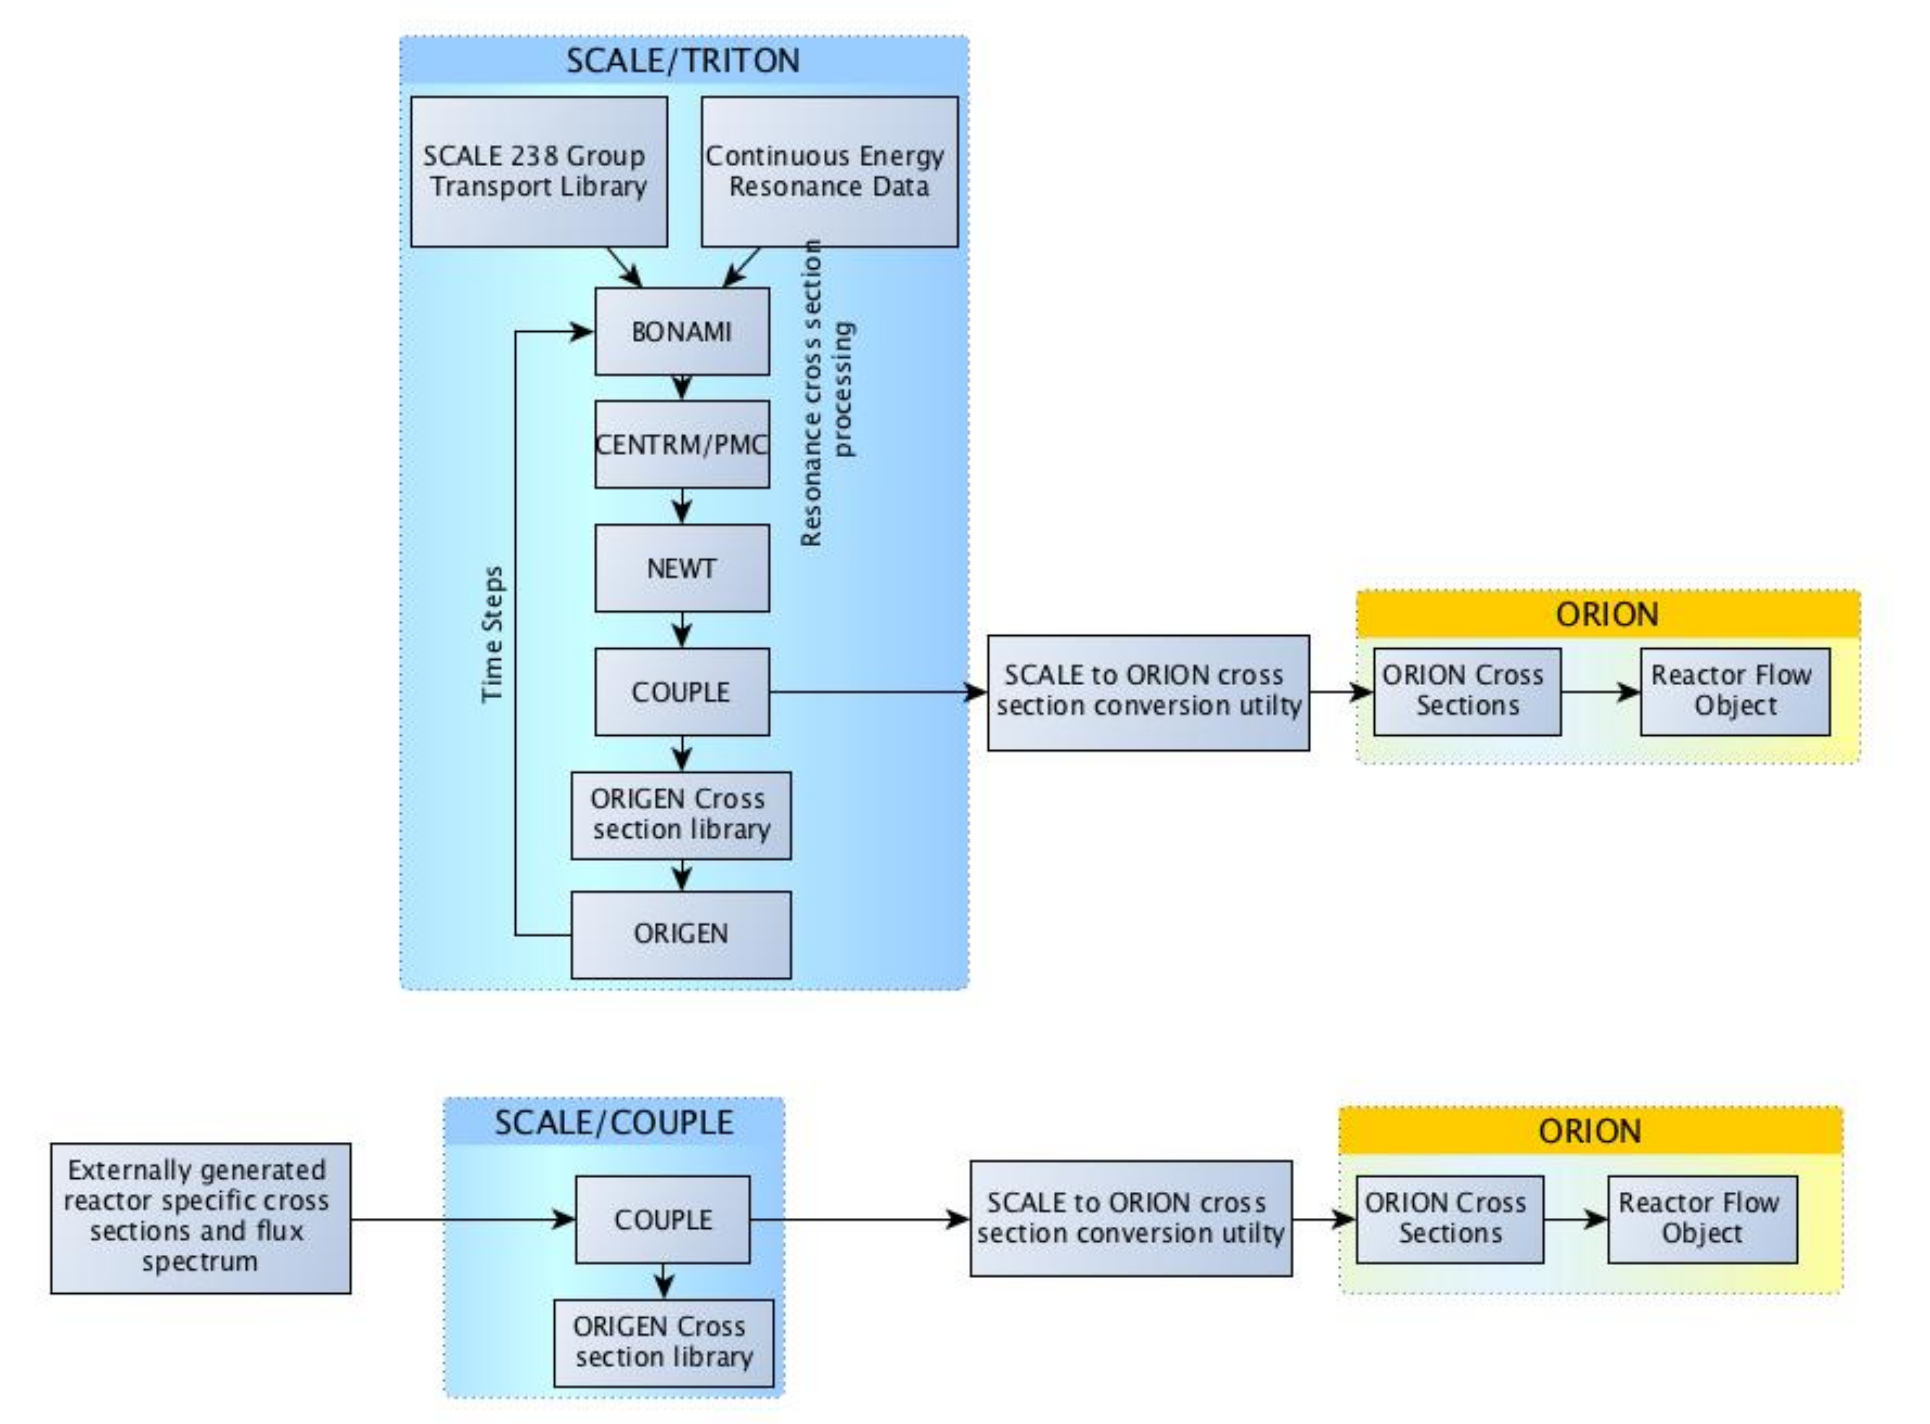
\includegraphics[scale=1.0]{./schematic.png}
        }
    \end{center}
    \caption{Schematic of link between SCALE and ORION}
    \label{fig:sch}
\end{figure}

In addition to generating cross sections, lattice physics codes can also be used to generate recipes, which are
tabulated isotopic fractions for a given fuel irradiation, used as transfer coefficients in ORION for each 
reactor and fuel type used. 

\section{Method}

A simple fuel cycle is created (shown in figure \ref{fig:flow}) where an \gls{MA} stream
(plutonium and americium with predefined isotopic composition) is mixed with a \gls{DU} (0.238\% $^{235}U$)
stream to create fuel for a single reactor. The fuel is then irradiated, using the MPR mode, to a predefined burnup (41.09 MWd/kgiHM for \gls{MOX} \gls{LWR}
and 100 MWd/kgiHM for \gls{SFR}) and then sent to the buffer. We report the fuel composition going into the
reactor and out of the reactor.

\begin{figure}[htbp!]
    \begin{center}
        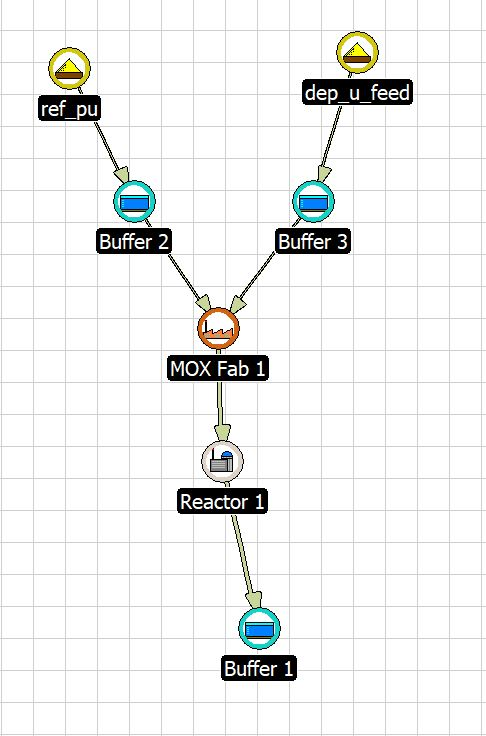
\includegraphics[scale=0.5]{./flow.jpg}
    \end{center}
    \caption{Material flow used for plutonium quality analysis.}
    \label{fig:flow}
\end{figure}

\subsection{Cross Section Generation}
For this test, we used a previously-generated cross section library as an input.
\gls{ORNL} has collaborated with \gls{NNL} to produce burnup-dependent cross section libraries specific to the fuel
cycles being evaluated in the FCO campaign \cite{wigeland_nuclear_2014}. The libraries are generated with the
SCALE suite of codes \cite{noauthor_scale_nodate}. The cross section for the \gls{PWR} \gls{MOX} model was generated from modeling
a Westinghouse 17 by 17 LOPAR fuel assembly in TRITON for 27 burnup steps and the cross section for the \gls{SFR}
model was generated from COUPLE using a steady-state flux spectrum from $MC^2-3 / REBUS-3$ \cite{lee_mc2-3:_2013}.
More details on cross section generation can be found in Peterson et al \cite{peterson_generating_2016}.


\section{Results}
The results of the \gls{FIT} are reproduced below. Note that all the results are for the fixed fraction
fuel fabrication because the \gls{FLM} for ORION is incomplete. The depletion calculations are similar to the
results from other codes. The main differences rise from the following two factors:

\begin{enumerate}
    \item Cross section generation
    \item `Lumping together' of driver and blanket region
\end{enumerate}

\subsection{\gls{MOX} \gls{LWR}}
Four qualities of \gls{MA} streams (ref, source one, two, three) are mixed with 
\gls{DU} (0.238\% $^{235}U$) in a fixed ratio (7\% \gls{MA}) and depleted in the thermal reactor
using the MPR mode in ORION. The charge and discharge fuel compositions are listed in
tables \ref{fig:lwr_charge} and \ref{fig:lwr_discharge}, respectively.

\begin{table}[h]
    \centering
    	\begin{tabular}{ccccc}
		\hline
		\textbf{wt\%} & \textbf{ref} & \textbf{source one} & \textbf{source two} & \textbf{source three} \\ 
		\hline
		U235 & 0.221 & 0.221 & 0.221 & 0.221 \\ 
		U238 & 92.77 & 92.77 & 92.77 & 92.77 \\ 
		PU238 & 0.138 & 0.218 & 0.200 & 0.279 \\ 
		PU239 & 4.357 & 3.611 & 3.289 & 2.697 \\ 
		PU240 & 1.574 & 1.702 & 2.373 & 1.719 \\ 
		PU241 & 0.559 & 0.822 & 0.317 & 1.112 \\ 
		PU242 & 0.349 & 0.562 & 0.764 & 0.894 \\ 
		AM241 & 0.018 & 0.082 & 0.053 & 0.296 \\ 
		Am+Pu & 6.999 & 6.999 & 6.999 & 6.999 \\ 
		\hline 
	\end{tabular} 

    \caption{Charge fuel composition for \gls{MOX} \gls{LWR}}
    \label{fig:lwr_charge}
\end{table}

\begin{table}[h]
    \centering
    	\begin{tabular}{c|ca|ca|ca|ca}
		\hline
		\textbf{wt\%} & \textbf{ref}  & \textbf{\% diff} & \textbf{1} & \textbf{\% diff} & \textbf{2} & \textbf{\% diff} & \textbf{3} & \textbf{\% diff}\\ 
		\hline
		\textbf{U234} & 0.002 & -4.07 & 0.002 & 33.14 & 0.003 & -4.35 & 0.005 & -4.89 \\ 
		\textbf{U235} & 0.117 & 0.065 & 0.108 & 5.815 & 0.099 & 6.339 & 0.099 & 8.988 \\ 
		\textbf{U236} & 0.023 & -1.03 & 0.024 & -2.50 & 0.026 & -6.29 & 0.026 & -6.32 \\ 
		\textbf{U238} & 90.51 & -0.40 & 89.89 & 0.193 & 89.85 & 0.051 & 89.86 & 0.076 \\ 
		\textbf{NP237} & 0.016 & -inf & 0.015 & -inf & 0.019 & -inf & 0.019 & -inf \\ 
		\textbf{PU236} & 0.0 & 0.0 & 0.0 & 0.0 & 0.0 & 0.0 & 0.0 & 0.0 \\ 
		\textbf{PU238} & 0.120 & 3.998 & 0.205 & 0.875 & 0.170 & 1.297 & 0.320 & 3.192 \\ 
		\textbf{PU239} & 2.255 & -0.55 & 2.175 & -10.7 & 1.836 & -5.43 & 1.760 & -5.97 \\ 
		\textbf{PU240} & 1.629 & -6.97 & 1.457 & 0.622 & 1.638 & 5.608 & 1.353 & -3.31 \\ 
		\textbf{PU241} & 0.862 & 4.373 & 0.910 & 1.680 & 0.953 & -1.49 & 0.863 & 4.151 \\ 
		\textbf{PU242} & 0.436 & 5.002 & 0.549 & 19.64 & 0.700 & 12.71 & 0.814 & 21.31 \\ 
		\textbf{AM241} & 0.059 & 5.982 & 0.078 & 2.161 & 0.069 & -8.99 & 0.116 & -0.51 \\ 
		\hline
		\hline
		\textbf{Am+Pu} & 5.486 & -3.19 & 5.592 & -4.95 & 5.611 & -2.83 & 5.526 & -3.21 \\ 
		\hline 
	\end{tabular} 

    \caption{Discharge fuel composition for \gls{MOX} \gls{LWR}}
    \label{fig:lwr_discharge}
\end{table}

\FloatBarrier

\subsection{\gls{SFR}}
Four qualities of \gls{SFR} streams (ref, source one, two, three) are mixed with
\gls{DU} (0.238\% $^{235}U$) in a fixed ratio (15.97\% \gls{MA}) and depleted in the 
fast reactor using the MPR mode in ORION. The charge and discharge fuel compositions are 
listed in tables \ref{fig:sfr_charge} and \ref{fig:sfr_discharge}, respectively.

Note that for the discharge compositions both the compositions depleted with driver
cross sections and blanket cross sections are listed. This is because two separate
cross section data are acquired for ORION, but the \gls{SFR} specification in the
FIT lumps the driver and blanket into one core. Given that difference, the depleted
composition should fall in between the depleted composition using the driver cross section (lower Pu+Am),
and the blanket cross section (higher Pu+Am).

\begin{table}[h]
    \centering
    	\begin{tabular}{ccccc}
		\hline
		\textbf{wt\%} & \textbf{ref} & \textbf{source one} & \textbf{source two} & \textbf{source three} \\ 
		\hline
		U235 & 0.199 & 0.199 & 0.199 & 0.199 \\ 
		U238 & 83.83 & 83.83 & 83.83 & 83.83 \\ 
		PU238 & 0.076 & 0.466 & 0.530 & 0.633 \\ 
		PU239 & 9.400 & 7.715 & 7.188 & 7.859 \\ 
		PU240 & 5.426 & 5.071 & 5.415 & 3.923 \\ 
		PU241 & 0.405 & 0.678 & 0.725 & 1.939 \\ 
		PU242 & 0.538 & 1.861 & 1.988 & 1.489 \\ 
		AM241 & 0.122 & 0.176 & 0.122 & 0.123 \\ 
		\hline
		\hline
		Am+Pu & 15.97 & 15.97 & 15.97 & 15.97 \\ 
		\hline 
	\end{tabular} 

    \caption{Charge fuel composition for \gls{SFR}}
    \label{fig:sfr_charge}
\end{table}

\begin{table}[h]
    \centering
    \resizebox{\textwidth}{!}{
    	\begin{tabular}{cccccccc}
		\hline
		\textbf{wt\%} & \textbf{ref blanket} & \textbf{ref driver} \textbf{one blanket} & \textbf{one driver} & \textbf{two blanket} & \textbf{two driver} & \textbf{three blanket} & \textbf{three driver} \\ 
		\hline
		U234 & 0.012 & 0.012 & 0.013 & 0.013 & 0.017 & 0.017 & 0.002 \\ 
		U235 & 0.090 & 0.058 & 0.088 & 0.057 & 0.094 & 0.063 & 0.092 \\ 
		U236 & 0.021 & 0.032 & 0.021 & 0.032 & 0.019 & 0.031 & 0.020 \\ 
		U238 & 76.30 & 72.79 & 76.18 & 72.61 & 76.72 & 73.53 & 76.66 \\ 
		Np237 & 0.0 & 0.0 & 0.0 & 0.0 & 0.0 & 0.0 & 0.0 \\ 
		PU236 & 0.0 & 0.0 & 0.0 & 0.0 & 0.0 & 0.0 & 0.0 \\ 
		PU238 & 0.267 & 0.286 & 0.284 & 0.296 & 0.368 & 0.386 & 0.072 \\ 
		PU239 & 7.684 & 9.503 & 7.461 & 9.342 & 7.783 & 9.559 & 8.415 \\ 
		PU240 & 4.310 & 5.429 & 4.515 & 5.609 & 3.519 & 4.605 & 4.692 \\ 
		PU241 & 0.537 & 0.819 & 0.569 & 0.859 & 0.841 & 0.928 & 0.485 \\ 
		PU242 & 1.521 & 1.601 & 1.615 & 1.698 & 1.316 & 1.431 & 0.479 \\ 
		AM241 & 0.201 & 0.186 & 0.180 & 0.174 & 0.300 & 0.245 & 0.152 \\ 
		Am+Pu & 14.67 & 18.10 & 14.78 & 18.27 & 14.24 & 17.38 & 14.34 \\ 
		\hline 
	\end{tabular} 
}
    \caption{Discharge fuel composition for \gls{SFR}}
    \label{fig:sfr_discharge}
\end{table}

\FloatBarrier

\section{Conclusion}
In-code fuel fabrication and depletion calculation capabilities are crucial
to modeling advanced fuel cycles.
Changes in the input stream can occur by multi-stage reprocessing or
technologies like on-line-reprocessing \glspl{MSR}. Using a fixed fraction method
for fuel fabrication and a recipe for depletion may work for a once-through cycle,
but can introduce large errors in advanced fuel cycles with continuous reprocessing.

We tested ORION's capability to perform depletion calculations
using cross sections and a user-defined power density. We showed that
the change in plutonium stream quality does affect the output depletion
from the reactor. However, the fuel loading model function in ORION is not tested
and is future work. Also, the \gls{SFR} discharge composition cannot be
compared directly, since the test \gls{SFR} uses a lumped-model \gls{SFR},
whereas the cross sections used for ORION separates the driver and the blanket fuel.

A better comparison could have been done if the analysts for different fuel cycle
codes used the same set of cross section data. However, it should be noted that
different codes use varying algorithms to perform fuel fabrication and depletion
calculations.


\bibliographystyle{unsrt}
\bibliography{bib}


\end{document}
